%% This manuscript uses the AASTeX v6.2 LaTeX 2e macros
%%
%% AASTeX is now based on Alexey Vikhlinin's emulateapj.cls
%% (Copyright 2000-2015).  See the classfile for details.

%% AASTeX requires revtex4-1.cls (http://publish.aps.org/revtex4/) and
%% other external packages (latexsym, graphicx, amssymb, longtable, and epsf).
%% All of these external packages should already be present in the modern TeX
%% distributions.  If not they can also be obtained at www.ctan.org.

%% The first piece of markup in an AASTeX v6.x document is the \documentclass
%% command. LaTeX will ignore any data that comes before this command. The
%% documentclass can take an optional argument to modify the output style.
%% The command below calls the preprint style  which will produce a tightly
%% typeset, one-column, single-spaced document.  It is the default and thus
%% does not need to be explicitly stated.
%%
%%
%% using aastex version 6.2
\documentclass{aastex62}

%% The default is a single spaced, 10 point font, single spaced article.
%% There are 5 other style options available via an optional argument. They
%% can be envoked like this:
%%
%% \documentclass[argument]{aastex62}
%%
%% where the layout options are:
%%
%%  twocolumn   : two text columns, 10 point font, single spaced article.
%%                This is the most compact and represent the final published
%%                derived PDF copy of the accepted manuscript from the publisher
%%  manuscript  : one text column, 12 point font, double spaced article.
%%  preprint    : one text column, 12 point font, single spaced article.
%%  preprint2   : two text columns, 12 point font, single spaced article.
%%  modern      : a stylish, single text column, 12 point font, article with
%% 		  wider left and right margins. This uses the Daniel
%% 		  Foreman-Mackey and David Hogg design.
%%  RNAAS       : Preferred style for Research Notes which are by design
%%                lacking an abstract and brief. DO NOT use \begin{abstract}
%%                and \end{abstract} with this style.
%%
%% Note that you can submit to the AAS Journals in any of these 6 styles.
%%
%% There are other optional arguments one can envoke to allow other stylistic
%% actions. The available options are:
%%
%%  astrosymb    : Loads Astrosymb font and define \astrocommands.
%%  tighten      : Makes baselineskip slightly smaller, only works with
%%                 the twocolumn substyle.
%%  times        : uses times font instead of the default
%%  linenumbers  : turn on lineno package.
%%  trackchanges : required to see the revision mark up and print its output
%%  longauthor   : Do not use the more compressed footnote style (default) for
%%                 the author/collaboration/affiliations. Instead print all
%%                 affiliation information after each name. Creates a much
%%                 long author list but may be desirable for short author papers
%%
%% these can be used in any combination, e.g.
%%
%% \documentclass[twocolumn,linenumbers,trackchanges]{aastex62}
%%
%% AASTeX v6.* now includes \hyperref support. While we have built in specific
%% defaults into the classfile you can manually override them with the
%% \hypersetup command. For example,
%%
%%\hypersetup{linkcolor=red,citecolor=green,filecolor=cyan,urlcolor=magenta}
%%
%% will change the color of the internal links to red, the links to the
%% bibliography to green, the file links to cyan, and the external links to
%% magenta. Additional information on \hyperref options can be found here:
%% https://www.tug.org/applications/hyperref/manual.html#x1-40003
%%
%% If you want to create your own macros, you can do so
%% using \newcommand. Your macros should appear before
%% the \begin{document} command.
%%
\newcommand{\vdag}{(v)^\dagger}
\newcommand\aastex{AAS\TeX}
\newcommand\latex{La\TeX}

% for non-stacked fractions
\newcommand{\sfrac}[2]{\mathchoice
  {\kern0em\raise.5ex\hbox{\the\scriptfont0 #1}\kern-.15em/
   \kern-.15em\lower.25ex\hbox{\the\scriptfont0 #2}}
  {\kern0em\raise.5ex\hbox{\the\scriptfont0 #1}\kern-.15em/
   \kern-.15em\lower.25ex\hbox{\the\scriptfont0 #2}}
  {\kern0em\raise.5ex\hbox{\the\scriptscriptfont0 #1}\kern-.2em/
   \kern-.15em\lower.25ex\hbox{\the\scriptscriptfont0 #2}}
  {#1\!/#2}}

\newcommand{\myhalf}{\sfrac{1}{2}}
\newcommand{\thalf}{\sfrac{3}{2}}

\newcommand{\eb}{{\bf{e}}}
\newcommand{\Ub}{{\bf{U}}}
\newcommand{\Ubt}{\widetilde{\Ub}}
\newcommand{\Vb}{{\bf{V}}}
\newcommand{\xb}{{\bf{x}}}

\newcommand{\dr}{\Delta r}
\newcommand{\dt}{\Delta t}

\newcommand{\etarho}{\eta_\rho}
\newcommand{\gammaonebar}{\overline{\Gamma}_1}
\newcommand{\Hnuc}{H_{\rm nuc}}
\newcommand{\omegadot}{\dot\omega}
\newcommand{\pred}{{\rm pred}}
\newcommand{\Sbar}{\overline{S}}

\newcommand{\inp}{\mathrm{in}}
\newcommand{\outp}{\mathrm{out}}
\newcommand{\nph}{{n+\myhalf}}
\newcommand{\nmh}{{n-\myhalf}}
\newcommand{\ow}{\overline{w_0}}
\newcommand{\dw}{\delta w_0}
\newcommand{\uadvone}{\Ub^{\mathrm{ADV},\star}}
\newcommand{\uadvonedag}{\Ub^{\mathrm{ADV},\dagger,\star}}
\newcommand{\uadvtwo}{\Ub^{\mathrm{ADV}}}
\newcommand{\uadvtwodag}{\Ub^{\mathrm{ADV},\dagger}}
\newcommand{\gcc}{\mathrm{g~cm^{-3} }}

% for the red MarginPars
\usepackage{color}
% make the MarginPars look pretty
\setlength{\marginparwidth}{0.5in}
\newcommand{\MarginPar}[1]{\marginpar{\vskip-\baselineskip\raggedright\tiny\sffamily
\hrule\smallskip{\color{red}#1}\par\smallskip\hrule}}

\usepackage{url}

\usepackage{mathtools}

%% Reintroduced the \received and \accepted commands from AASTeX v5.2
\received{XXX X, XXXX}
\revised{XXX X, XXXX}
\accepted{XXX X, XXXX}
%% Command to document which AAS Journal the manuscript was submitted to.
%% Adds "Submitted to " the arguement.
\submitjournal{ApJ}

%% Mark up commands to limit the number of authors on the front page.
%% Note that in AASTeX v6.2 a \collaboration call (see below) counts as
%% an author in this case.
%
%\AuthorCollaborationLimit=3
%
%% Will only show Schwarz, Muench and "the AAS Journals Data Scientist
%% collaboration" on the front page of this example manuscript.
%%
%% Note that all of the author will be shown in the published article.
%% This feature is meant to be used prior to acceptance to make the
%% front end of a long author article more manageable. Please do not use
%% this functionality for manuscripts with less than 20 authors. Conversely,
%% please do use this when the number of authors exceeds 40.
%%
%% Use \allauthors at the manuscript end to show the full author list.
%% This command should only be used with \AuthorCollaborationLimit is used.

%% The following command can be used to set the latex table counters.  It
%% is needed in this document because it uses a mix of latex tabular and
%% AASTeX deluxetables.  In general it should not be needed.
%\setcounter{table}{1}

%%%%%%%%%%%%%%%%%%%%%%%%%%%%%%%%%%%%%%%%%%%%%%%%%%%%%%%%%%%%%%%%%%%%%%%%%%%%%%%%
%%
%% The following section outlines numerous optional output that
%% can be displayed in the front matter or as running meta-data.
%%
%% If you wish, you may supply running head information, although
%% this information may be modified by the editorial offices.
\shorttitle{MAESTROeX Low Mach Number Astrophysics}
\shortauthors{Fan et al.}
%%
%% You can add a light gray and diagonal water-mark to the first page
%% with this command:
% \watermark{text}
%% where "text", e.g. DRAFT, is the text to appear.  If the text is
%% long you can control the water-mark size with:
%  \setwatermarkfontsize{dimension}
%% where dimension is any recognized LaTeX dimension, e.g. pt, in, etc.
%%
%%%%%%%%%%%%%%%%%%%%%%%%%%%%%%%%%%%%%%%%%%%%%%%%%%%%%%%%%%%%%%%%%%%%%%%%%%%%%%%%

%% This is the end of the preamble.  Indicate the beginning of the
%% manuscript itself with \begin{document}.

\begin{document}

\title{MAESTROeX: A Massively Parallel Low Mach Number Astrophysical Solver}

%% LaTeX will automatically break titles if they run longer than
%% one line. However, you may use \\ to force a line break if
%% you desire. In v6.2 you can include a footnote in the title.

%% A significant change from earlier AASTEX versions is in the structure for
%% calling author and affilations. The change was necessary to implement
%% autoindexing of affilations which prior was a manual process that could
%% easily be tedious in large author manuscripts.
%%
%% The \author command is the same as before except it now takes an optional
%% arguement which is the 16 digit ORCID. The syntax is:
%% \author[xxxx-xxxx-xxxx-xxxx]{Author Name}
%%
%% This will hyperlink the author name to the author's ORCID page. Note that
%% during compilation, LaTeX will do some limited checking of the format of
%% the ID to make sure it is valid.
%%
%% Use \affiliation for affiliation information. The old \affil is now aliased
%% to \affiliation. AASTeX v6.2 will automatically index these in the header.
%% When a duplicate is found its index will be the same as its previous entry.
%%
%% Note that \altaffilmark and \altaffiltext have been removed and thus
%% can not be used to document secondary affiliations. If they are used latex
%% will issue a specific error message and quit. Please use multiple
%% \affiliation calls for to document more than one affiliation.
%%
%% The new \altaffiliation can be used to indicate some secondary information
%% such as fellowships. This command produces a non-numeric footnote that is
%% set away from the numeric \affiliation footnotes.  NOTE that if an
%% \altaffiliation command is used it must come BEFORE the \affiliation call,
%% right after the \author command, in order to place the footnotes in
%% the proper location.
%%
%% Use \email to set provide email addresses. Each \email will appear on its
%% own line so you can put multiple email address in one \email call. A new
%% \correspondingauthor command is available in V6.2 to identify the
%% corresponding author of the manuscript. It is the author's responsibility
%% to make sure this name is also in the author list.
%%
%% While authors can be grouped inside the same \author and \affiliation
%% commands it is better to have a single author for each. This allows for
%% one to exploit all the new benefits and should make book-keeping easier.
%%
%% If done correctly the peer review system will be able to
%% automatically put the author and affiliation information from the manuscript
%% and save the corresponding author the trouble of entering it by hand.

\correspondingauthor{Doreen Fan; DFan@lbl.gov}

\author[0000-0002-3246-4315]{Duoming Fan}
\affil{Lawrence Berkelely National Laboratory \\
Center for Computational Sciences and Engineering \\
One Cyclotron Road, MS 50A-3111 \\
Berkeley, CA 94720, USA}

\author[0000-0003-1791-0265]{Andrew Nonaka}
\affil{Lawrence Berkelely National Laboratory \\
Center for Computational Sciences and Engineering \\
One Cyclotron Road, MS 50A-3111 \\
Berkeley, CA 94720, USA}

\author[0000-0003-2103-312X]{Ann S. Almgren}
\affil{Lawrence Berkelely National Laboratory \\
Center for Computational Sciences and Engineering \\
One Cyclotron Road, MS 50A-3111 \\
Berkeley, CA 94720, USA}

\author[0000-0002-1530-781X]{Alice Harpole}
\affil{Stony Brook University \\
Department of Physics and Astronomy \\
Stony Brook, NY 11794-3800, USA}

\author[0000-0001-8401-030X]{Michael Zingale}
\affil{Stony Brook University \\
Department of Physics and Astronomy \\
Stony Brook, NY 11794-3800, USA}


%% Note that the \and command from previous versions of AASTeX is now
%% depreciated in this version as it is no longer necessary. AASTeX
%% automatically takes care of all commas and "and"s between authors names.

%% AASTeX 6.2 has the new \collaboration and \nocollaboration commands to
%% provide the collaboration status of a group of authors. These commands
%% can be used either before or after the list of corresponding authors. The
%% argument for \collaboration is the collaboration identifier. Authors are
%% encouraged to surround collaboration identifiers with ()s. The
%% \nocollaboration command takes no argument and exists to indicate that
%% the nearby authors are not part of surrounding collaborations.

%% Mark off the abstract in the ``abstract'' environment.
\begin{abstract}
We present MAESTROeX, a massively parallel solver for low Mach number astrophysical flows.
Our model equations allow for long-time integration for highly subsonic flows compared to compressible approaches.
The code leverages the new AMReX framework for block-structured adaptive mesh refinement calculations, and also provides additional algorithmic features from the original MAESTRO code.
We present a new temporal integration option that is much simpler than our previous approach while retaining the same order order of accuracy.
We also provide a more accurate spatial discretization for mapping the base state onto the full state Cartesian grid.
Using our previous studies on the convective phase of single-degenerate progenitor models of Type Ia supernovae, we characterize the performance of the code and validate the new algorithmic features.
\end{abstract}

%% Keywords should appear after the \end{abstract} command.
%% See the online documentation for the full list of available subject
%% keywords and the rules for their use.
\keywords{convection, hydrodynamics, methods: numerical, nuclear reactions, nucleosynthesis, abundances, supernovae: general}

%% From the front matter, we move on to the body of the paper.
%% Sections are demarcated by \section and \subsection, respectively.
%% Observe the use of the LaTeX \label
%% command after the \subsection to give a symbolic KEY to the
%% subsection for cross-referencing in a \ref command.
%% You can use LaTeX's \ref and \label commands to keep track of
%% cross-references to sections, equations, tables, and figures.
%% That way, if you change the order of any elements, LaTeX will
%% automatically renumber them.
%%
%% We recommend that authors also use the natbib \citep
%% and \citet commands to identify citations.  The citations are
%% tied to the reference list via symbolic KEYs. The KEY corresponds
%% to the KEY in the \bibitem in the reference list below.

\section{Introduction} \label{sec:intro}

TODO list:
\begin{itemize}
\item Weak scaling tests of original algorithm, comparing MAESTRO to MAESTROeX.  Use cori knl, 4 MPI per node, 16 threads per MPI
\item Run at effective $512^3$ resolution (maybe to ignition?... need to see how max T trends go) (1) classic MAESTRO, (2) MAESTROeX with original algorithm, (3) MAESTROeX with new temporal integrator, (4) MAESTROeX with new temporal integrator and irregular dr, (5) MAESTROeX with original algorithm and 3-levels of AMR, (6) MAESTROeX with new temporal integrator and 3 levels of AMR.
\item (perhaps) a demonstration of what goes wrong when you don't split the velocity dynamics in the projection
\end{itemize}

Many astrophysical flows are highly subsonic; sound waves carry sufficiently little energy that they do not significantly affect the convective dynamics of the system.
In many of these flows, modeling long-time convective dynamics are of interest, and numerical approaches based on compressible hydrodynamics are intractable, even on modern supercomputers.
One approach to this problem is to use low Mach number models.
In a low Mach number approach, sound waves are eliminated from the governing equations while retaining compressibilitiy effects due to, e.g., nuclear energy release, compositional changes, and thermal diffusion.
The resulting model can be numerically integrated with much larger time steps than a compressible model.
Low Mach number models have been developed for a variety of contexts including combustion \citep{day2000numerical}, terrestrial atmospheric modeling \citep{duarte2015low}, 
and elastic solids \citep{abbate2017all}.

Previously, we developed the low Mach number astrophysical solver, MAESTRO.
The low Mach number model in MAESTRO is unique in that it is specifically designed for astrophysical settings with significant atmospheric stratification.
Central to the algorithm is a stratified background (or base) state density and pressure held in hydrostatic equilibrium, and also vary as a function of altitude and time.
MAESTRO is a structured-grid, finite-volume code that utlizes adaptive mesh refinement (AMR) to refine grids locally in space.
MAESTRO is suitable for for full spherical stars, as well as planar simulations of dynamics within localized regions of a star.

The key numerical developments of the original MAESTRO algorithm are presented in a series of papers which we refer to as Papers I-V:
\begin{itemize}
\item In Paper I \citep{MAESTRO_I}, we derive the low Mach number equation set from the fully compressible equations.
\item In Paper II \citep{MAESTRO_II}, we incorporate the effects atmospheric expansion through the use of a time-dependent background state.
\item In Paper III \citep{MAESTRO_III}, we incorporate reactions and the associated coupling to the hydrodynamics.
\item In Paper IV \citep{MAESTRO_IV}, we describe our treatment of spherical stars in a three-dimensional Cartesian geometry.
\item In Paper V \citep{MAESTRO_V}, we describe the use of block-structured adaptive mesh refinement to focus spatial resolution in regions of interest.
\end{itemize} 

Since then, there have been many scientific investigations using MAESTRO, which include additional algorithmic enhancements.  Topics include:
\begin{itemize}
\item The convective phase preceding Chandrasekhar mass models for type Ia supernovae \citep{MAESTRO_convection,MAESTRO_AMR,MAESTRO_CASTRO}.
\item Convection in massive stars \citep{Gilet:2013}.
\item Sub-Chandrasekhar white dwarfs \citep{subChandra_I,subChandra_II}.
%  In the latter paper we introduced an optional modification to the momentum equation of velocity constraint that conserves total energy, can give results closer to compressible codes of convective dynamics, including low density regions at the surface of a star.
\item Type I X-ray bursts \citep{XRB_I,XRB_II,XRB_III}.
%  In \cite{XRB_I} we discuss the modifications required for implicit thermal conduction, as well as an additional ``volume discrepancy'' modification to the velocity constraint to force the species and enthalpy to evolve in a manner consistent with the background pressure.
\end{itemize}

We also present new algorithmic methodology that improves upon Paper V in a number of ways.
First, the overall temporal algorithm has been greatly simplified without compromising accuracy.
The key design decision was to replace the predicted evolution of the base state with 
a predictor-corrector approach.  Not only does this greatly simplify the dynamics of the base
state, but this treatment is more amenable to higher-order multiphysics coupling strategies
based on method-of-lines integration.  Second, we now provide additional spatial mapping
procedures that reduces, and in some cases eliminates, mapping error from the one-dimensional
base state to the Cartesian grid state for spherical problems.
Finally, the code has been completely ported to a new software framework suitable for modern manycore supercomputers.
The resulting MAESTROeX is implemented in the C++/F90 AMReX software library.  MAESTROeX uses MPI+OpenMP parallelism
and scales to XXX MPI processes, each capable of spawning tens of threads.
\MarginPar{quantify XXX.  I think it's 5,000-10,000 MPIs with potentially hundreds of threads}

The resulting code is publicly available on GitHub at {\url https://github.com/AMReX-Astro/MAESTROeX} and uses the microphysics 
libraries at {\url https://github.com/starkiller-astro/Microphysics} and the AMReX software library for block-structured adaptive mesh refinement
{\url https://github.com/AMReX-Codes/amrex}.


\section{Governing Equations}\label{sec:equations}
Low Mach number models for reacting flow were originally derived using asymptotic analysis
\citep{rehm1978equations,majda1985derivation} and used in terrestrial combustion applications
\citep{knio1999semi,day2000numerical}.  These models have been extended to nuclear flames
in astrophysical environments using adaptive algorithms in space and time \citep{Bell:2004}.
In Papers I-III, we extended this work by deriving a model and algorithm suitable for stratified astrophysical flow.
In our model, we take the standard equations of reacting, compressible flow, and recast the equation
of state (EOS) as a divergence constraint on the velocity field.
The resulting model is a series of evolution equations for mass, momentum, and energy, subject
to to an additional constraint on velocity.  The evolution equations are
\begin{eqnarray}
\frac{\partial\Ub}{\partial t} &=& -\Ub\cdot\nabla\Ub  - \frac{1}{\rho}\nabla\pi - \frac{\rho-\rho_0}{\rho} g\eb_r,\label{eq:momentum}\\
\frac{\partial(\rho X_k)}{\partial t} &=& -\nabla\cdot(\rho X_k\Ub) + \rho\omegadot_k,\label{eq:species}\\
\frac{\partial(\rho h)}{\partial t} &=& -\nabla\cdot(\rho h\Ub) + \frac{Dp_0}{Dt} + \rho\Hnuc.\label{eq:enthalpy}
\end{eqnarray}
Here $\rho$, $\Ub$, and $h$ are the mass density,
velocity and specific enthalpy, respectively, and
$X_k$ are the mass fractions of species $k$ with associated
production rate $\omegadot_k$.  The species are constrained
such that $\sum_k X_k = 1$ giving $\rho = \sum_k (\rho X_k)$ and
\begin{equation}
\frac{\partial\rho}{\partial t} = -\nabla\cdot(\rho\Ub).
\end{equation}
Here $\Hnuc$ is the nuclear energy generation rate per unit mass.
The total pressure is decomposed into a one-dimensional hydrostatic base state
 pressure, $p_0 = p_0(r,t)$, and a dynamic pressure, $\pi = \pi(\xb,t)$, such that 
$p = p_0 + \pi$ and $|\pi|/p_0 = \mathcal{O}({\rm Ma}^2)$ (we use $\xb$ to represent the Cartesian coordinate 
directions of the full state and $r$ to represent the radial coordinate direction for 
the base state).  We also define a one-dimensional base state density, $\rho_0 = \rho_0(r,t)$, that represents the lateral average (see Section \ref{Sec:Spatial}) of $\rho$ and is in hydrostatic equilibrium with $p_0$, i.e., 
\begin{equation}
\nabla p_0 = -\rho_0 g\eb_r, \label{eq:HSE}
\end{equation}
where $g=g(r,t)$ is the magnitude of the gravitational acceleration and $\eb_r$ is the unit vector in the outward radial direction. 
Thermal diffusion is not discussed in this paper, but we have previously described the modifications to the original algorithm required 
for implicit thermal diffusion in \cite{XRB_I}; inclusion of these effects in the new algorithm presented here is straightforward.

Mathematically, equations (\ref{eq:momentum})-(\ref{eq:enthalpy}) must still be closed by the EOS.  
This is done by taking the Langrangian derivative of the EOS for pressure as a function of the thermodynamic variables, 
substituting in the equations of motion for mass and energy,
and requiring that the pressure is a prescribed function of altitude and time based on the hydrostatic equilibrium condition.
See Papers I and II for details of this derivation.
The resulting equation is a divergence constraint on the velocity field,
\begin{equation}
\nabla\cdot(\beta_0\Ub) = \beta_0\left(S - \frac{1}{\gammaonebar p_0}\frac{\partial p_0}{\partial t}\right).\label{eq:U divergence}
\end{equation}
Here $\beta_0$ is a density-like variable that carries background stratification, defined as
\begin{equation}
\beta_0(r,t) = \rho_0(0,t)\exp\left(\int_0^r\frac{1}{\gammaonebar p_0}\frac{\partial p_0}{\partial r'}dr'\right),
\end{equation}
where $\gammaonebar$ is the lateral average of $\Gamma_1 = d(\log p)/d(\log\rho)$ at constant entropy.
The expansion term, $S$, incorporates local compressibility effects due to compositional changes and heat release from reactions,
\begin{equation}
S = -\sigma\sum_k\xi_k\omegadot_k + \frac{1}{\rho p_\rho}\sum_k p_{X_k}\omegadot_k + \sigma\Hnuc,\label{eq:S}
\end{equation}
where $p_{X_k} \equiv \left. \partial p / \partial X_k
\right|_{\rho,T,X_{j,j\ne k}}$, $\xi_k \equiv \left. \partial h /
\partial X_k \right |_{p,T,X_{j,j\ne k}},
p_\rho \equiv \left.
\partial p/\partial \rho \right |_{T, X_k}$, and $\sigma \equiv
p_T/(\rho c_p p_\rho)$, with $p_T \equiv \left. \partial p / \partial
T \right|_{\rho, X_k}$ and $c_p \equiv \left.  \partial h / \partial T
\right|_{p,X_k}$ is the specific heat at constant pressure.

To summarize, we model evolution equations for momentum, mass, and energy, (\ref{eq:momentum})-(\ref{eq:enthalpy}) subject to a divergence constraint on the velocity (\ref{eq:U divergence}) and the hydrostatic equilibrium condition (\ref{eq:HSE}).


\section{Numerical Algorithm}

\subsection{Spatial Discretization}\label{Sec:Spatial}
MAESTRO contains variables defined on Cartesian grids 
one-dimensional base state stored on radial arrays.

 associated with square (in 2D) or cubic (in 3D)


(description of base state mapping in planar, and origianl spherical, and new spherical)

Mapping from the base state to the full state


Mapping a Cartesian variable to a one-dimensional radial array uses the lateral averating operator.

One of the key numerical modules is the ``lateral average'', which computes the average over a 
layer of a Cartesian grid variable onto a one-dimensional radial array.
In planar geometries, this is a straightforward arithmetic average of cells at
a particular height since the radial cell centers are in alignment
with the Cartesian grid cell centers.
However for spherical problems, the procedure is much more complicated.
In Section 4 of Paper V, we describe how there is a finite, easily computable set of radii that any Cartesian cell-center can map to.  
Specifically, for every Cartesian cell, there exists an integer $m$ such that the radius to the center of the star is given by $\hat{r}_m=\Delta x\sqrt{0.75+2m}$.
We average by binning all the cells associated with each radii and taking the average.
Then we interpolate this data onto a one-dimensional radial array.  Previously, MAESTRO only allowed for radial arrays with a constant $\Delta r$ (typically equal to $\Delta x/5$.
Here we present a new option to retain an irregularly-spaced radial array to eliminate mapping errors back onto the Cartesian grid state.
Consider a spherical star in hydrostatic equlibrium at rest.  In the absense of reactions, the star should remain at rest.
The buoyancy forcing term in the momentum equation contains $\rho-\rho_0$.  With the original scheme, interpolation errors in computing $\rho_0$ by averaging would cause artifical acceleration in the velocity field due to the interpolation error from the Cartesian grid to and from the radial base state.  By retaining the radial base state as an irregularly spaced array, the effects due to interpolation error are completely eliminated.


\subsection{Temporal Integration Scheme}\label{Sec:Temporal Integration Scheme}
Previously we adopted an approach where we split the velocity into a base state component, $w_0(r,t)$, 
and a local velocity $\Ubt(\xb,t)$, so that
\begin{equation}
\Ub = \Ubt(\xb,t) + w_0(r,t)\eb_r,
\end{equation}
We used $w_0$ to provide an estimate of the base state density evolution over a time step.

Our new temporal integration scheme does not use this splitting, and is much simpler than the scheme from Paper V.
In this new scheme we use a simpler, predictor-corrector approach to the base state density and pressure that no longer requires the complex algorithm from Paper V, yet still retains the same overall second-order accuracy.
Also, we now evolve the full-state velocity directly rather than the perturbational velocity, eliminating the need to compute additional forcing terms that arise due to the splitting.

We now describe the new temporal integration scheme, which has been greatly simplified
from Paper V without formal loss of order of accuracy.
Note that this temporal integration scheme is valid for the original base state mapping (with constant base state grid spacing), or the new irregularly spaced base state mapping.

At the beginning of each time step we have the cell-centered state,
$(\Ub,\rho X_k,\rho h,\rho_0,p_0)^n$, and nodal state, $\pi^{n-\myhalf}$.
At any time, the associated density, composition, and enthalpy can be trivially computed using, e.g.,
\begin{equation}
\rho^n = \sum_k(\rho X_k)^n, \quad
X_k^n = (\rho X_k)^n / \rho^n, \quad
h^n = (\rho h)^n / \rho^n.
\end{equation}
Temperature is computed using the equation of state, e.g.,
\footnote{As described in Paper V, for planar problems we compute temperature using $h$ instead of $p_0$, since we have successfully developed planar volume discrepancy schemes to effectively couple the enthalpy to the rest of the solution; see \cite{XRB_I}.  We are still exploring this option for spherical stars.}
\begin{equation}
T = T(\rho,p_0,X_k),
\end{equation}
and ($\gammaonebar,\beta_0)$ are computed from $(\rho,p_0,X_k)$ (see Appendix A of Paper I and Appendix C of Paper III for details).

The overall flow of the algorithm is a second-order Strang splitting approach for the coupling of the reactions and advection of the thermodynamic variables.  
We use a predictor-corrector approach within the Strang splitting scheme to achieve second-order accuracy in time.
We integrate the velocity using a standard second-order projection method to enforce the divergence constraint.
To summarize:
\begin{itemize}
\item In {\bf Step 1} we react the thermodynamic variables over $\Delta t/2$.
\item In {\bf Steps 2-4} we advect the thermodynamic variables over $\Delta t$.  Specifically, we compute an estimate for the expansion term, $S$, project the face-centered, time-centered velocities so they satisfy the divergence constraint, and then advect the thermodynamic variables.
\item In {\bf Step 5} we react the thermodynamic variables over $\Delta t/2$.\footnote{After this step we could skip to the velocity advance in {\bf Steps 10-11}, however the overall scheme would be only first-order in time, so {\bf Steps 6-9} can be thought of as a trapezoidal corrector step.}
\item In {\bf Steps 6-8} we redo the advection in {\bf Steps 2-4} but are able to use the trapezoidal rule to time-center certain quantities such as $S$, $\rho_0$, etc.
\item In {\bf Step 9} we redo the reactions from {\bf Step 5} using the improved results for the corrector advection step.
\item In {\bf Steps 10-11} we and update the velocity, compute the expansion term, $S$, and project the cell-centered velocities.
\end{itemize}

There are a few key numerical modules we use in each time step.
\begin{itemize}
\item {\bf Average}$[\phi]\rightarrow[\overline\phi]$ computes the lateral average of a quantity over a layer at constant radius $r$, as described above in Section \ref{Sec:Spatial}.
\item {\bf Enforce HSE}$[\rho_0]\rightarrow[p_0]$ computes the base state pressure, $p_0$, from a base state density, $\rho_0$ by integrating the hydrostatic equilibrium condition in 1D (see equation (A10) in Paper V).  The base state pressure remains equal to a constant value from the location of a prescribed cutoff density outward for the entire simulation.
\item {\bf React State}$[(\rho X_k)^{\rm in},(\rho h)^{\rm in},p_0]\rightarrow[(\rho X_k)^{\rm out},(\rho h)^{\rm out},(\rho\dot\omega),(\rho\Hnuc)]$ integrates the species and enthalpy due to reactions over $\Delta t/2$ by solving
\begin{equation}
\frac{dX_k}{dt} = \dot\omega_k(\rho,X_k,T); \qquad
\frac{dT}{dt} = \frac{1}{c_p}\left(-\sum_k\xi_k\dot\omega_k + H_{\rm nuc})\right)
\end{equation}
The inputs are the species, enthalpy, and base state pressure, and the outpus are the species, enthalpy, reaction rates, and nuclear energy generation rate.
See Papers III and V for details.
\end{itemize}

Each time step satisfies the standard advective CFL condition,
\begin{equation}
\Delta t = \sigma^{\rm CFL} \min_i(\Delta x / U_i),
\end{equation}
where for our simulations we typically use $\sigma^{\rm CFL}\sim 0.5$.
There are additional constraints on the timestep that are typically much less restrictive than the advective CFL including
the acceleration due to the buoyancy force (sometimes in effect when the velocity is approximately zero at the start of some simulations) 
and the local magnitude of the divergence constraint (to prevent too much mass evacuation from a cell in a time step); see Section 3.4 in Paper III for details.

At the beginning of each simulation, we define $(\Ub,\rho X_k,\rho h)$...

\MarginPar{mention cutoff densities}

\begin{description}

%--------------------------------------------------------------------------
% STEP 1
%--------------------------------------------------------------------------
\item[Step 1] {\em React the full state through the first time interval of $\dt / 2.$}

Call {\bf React State}$[(\rho X_k)^n, (\rho h)^n, p_0^n] \rightarrow [(\rho X_k)^{(1)}, (\rho h)^{(1)}, (\rho \omegadot_k)^{(1)}, (\rho \Hnuc)^{(1)}]$.

%--------------------------------------------------------------------------
% STEP 2
%--------------------------------------------------------------------------

\item[Step 2] {\em Compute the provisional time-centered expansion,
    $S^{\nph,\star}$.}

We compute an estimate for the time-centered expansion term in the velocity
divergence constraint.  Following \citet{Bell:2004}, we extrapolate
to the half-time using $S$ at the previous and current
time steps,
\begin{equation}
S^{\nph,\star} = S^n + \frac{\dt^n}{2} \left(\frac{S^n - S^{n-1}}{\dt^{n-1}}\right).
\end{equation}
Note that in the first time step we average $S^0$ and $S^1$ from the
initialization step.

%--------------------------------------------------------------------------
% STEP 3
%--------------------------------------------------------------------------
\item[Step 3] {\em Construct the provisional time-centered advective velocity on
edges, $\uadvone$.}

The construction of face-centered time-centered states used to discretize the
advection terms for velocity, species, and enthalpy, are performed using
a standard multidimensional corner transport upwind approach
\citep{colella1990multidimensional,saltzman1994unsplit} with piecewise-parabolic
one-dimensional tracing \citep{colella1984piecewise}.  The full details of this
Godunov advection approach for all steps in this algorithm are described 
in Appendix A of \cite{XRB_III}.

In this step, using equation (\ref{eq:momentum}), 
we compute time-centered edge velocities, $\uadvonedag$, using
$\Ub^n$.  The $\dagger$ superscript refers to the
fact that the predicted velocity field does not satisfy the divergence
constraint.  We then construct $\uadvone$ from $\uadvonedag$
using a MAC projection.
We note that $\uadvone$ satisfies the divergence constraint
\begin{equation}
\nabla \cdot \left(\beta_0^n \uadvone\right) = \beta_0^n \left[S^{\nph,\star} - \frac{1}{\gammaonebar^np_0^n}\left(\frac{\partial p_0}{\partial t}\right)^{n-\myhalf} \right].\label{eq:div1}
\end{equation}
In practice we solve for.

%--------------------------------------------------------------------------
% STEP 4
%--------------------------------------------------------------------------
\item[Step 4] {\em Advect the full state through a time interval of $\dt.$}

\begin{enumerate}
\renewcommand{\theenumi}{{\bf \Alph{enumi}}}

\item Update $(\rho X_k)$ using a discretized version of
%
\begin{equation}
\frac{\partial(\rho X_k)}{\partial t} = -\nabla\cdot(\rho X_k\Ub) + \rho\omegadot_k,
\end{equation}
%
omitting the reaction terms, which were already
accounted for in {\bf React State}.  The update consists of two steps:

\begin{enumerate}
\renewcommand{\labelenumii}{{\bf \roman{enumii}}.}

\item Compute the time-centered species edge states, $(\rho X_k)^{\nph,\pred}$,
  for the conservative update of $(\rho X_k)^{(1)}$ using a Godunov approach \citep{XRB_III}.
\MarginPar{mention $\rho'$ and $X$ advection; $(\rho h)'$ advection}

\item Evolve $(\rho X_k)^{(1)} \rightarrow (\rho X_k)^{(2),\star}$ using
\begin{equation}
(\rho X_k)^{(2),\star} = (\rho X_k)^{(1)}
  - \dt \left\{ \nabla \cdot \left[ \uadvone (\rho X_k)^{\nph,\pred} \right] \right\},
\end{equation}

\end{enumerate}

\item Update $\rho_0$ by calling {\bf Average}$[\rho^{(2),\star}]\rightarrow[\rho_0^{n+1,\star}]$.

\item Update $p_0$ by calling {\bf Enforce HSE}$[\rho_0^{n+1,\star}] \rightarrow [p_0^{n+1,\star}]$.

\item Update the enthalpy using a discretized version of equation
%
\begin{equation}
\frac{\partial(\rho h)}{\partial t} = -\nabla\cdot(\rho h\Ub) + \frac{Dp_0}{Dt} + \rho\Hnuc,
\end{equation}
%
again omitting the reaction and heating terms
since we already accounted for
them in {\bf React State}.  This equation takes the form:
\begin{equation}
\frac{\partial (\rho h)}{\partial t}  = - \nabla \cdot (\Ub \rho h) + \frac{\partial p_0}{\partial t} + (\Ub \cdot \eb_r) \frac{\partial p_0}{\partial r}.
\end{equation}
For spherical geometry, we solve the
analytically equivalent form,
\begin{equation}
\frac{\partial (\rho h)}{\partial t}  = - \nabla \cdot (\Ub \rho h) + \frac{\partial p_0}{\partial t} + \nabla \cdot (\Ub p_0) - p_0 \nabla \cdot \Ub.
\end{equation}
The update consists of two steps:

\begin{enumerate}
\renewcommand{\labelenumii}{{\bf \roman{enumii}}.}

\item Compute the time-centered enthalpy edge state, $(\rho h)^{\nph,\pred},$
  for the conservative update of $(\rho h)^{(1)}$
  using using a Godunov approach \citep{XRB_III}.

\item Evolve $(\rho h)^{(1)} \rightarrow (\rho h)^{(2),\star}$.
\begin{description}
\item For planar geometry,
\begin{eqnarray}
(\rho h)^{(2),\star}
&=& (\rho h)^{(1)} \nonumber \\
&&- \dt \left\{ \nabla \cdot \left[ \uadvone (\rho h)^{\nph,\pred} \right] \right\} \nonumber \\
&& + \left(p_0^{n+1,*} - p_0^n\right) \nonumber \\
&& + \dt \left(\uadvone \cdot \eb_r\right) \left(\frac{\partial p_0}{\partial r} \right)^{n}
\end{eqnarray}

\item For spherical geometry,
\begin{eqnarray}
(\rho h)^{(2),\star}
&=& (\rho h)^{(1)} \nonumber \\
&&- \dt \left\{ \nabla \cdot \left[ \uadvone (\rho h)^{\nph,\pred} \right] \right\} \nonumber \\
&& + \left(p_0^{n+1,*} - p_0^n\right) \nonumber \\
&& + \dt \left \{ \nabla \cdot \left (\uadvone p_0^{n+\myhalf} \right ) - p_0^{n+\myhalf} \nabla \cdot \uadvone \right \}
\end{eqnarray}
\end{description}
where we define $p_0^\nph$ as $p_0^\nph = (p_0^n+p_0^{n+1,*})/2$.

\end{enumerate}
Note that outside the cutoff density region, we compute enthalpy using the EOS.

\end{enumerate}

%--------------------------------------------------------------------------
% STEP 5
%--------------------------------------------------------------------------
\item[Step 5] {\em React the full state through a second time interval of $\dt / 2.$}

Call {\bf React State}$[ (\rho X_k)^{(2),\star}, (\rho h)^{(2),\star}, p_0^{n+1,\star}] 
\rightarrow 
[ (\rho X_k)^{n+1,\star}, (\rho h)^{n+1,\star}, (\rho \omegadot_k)^{n+1,\star}, (\rho \Hnuc)^{n+1,\star} ].$

%--------------------------------------------------------------------------
% STEP 6
%--------------------------------------------------------------------------
\item[Step 6] {\em Compute the time-centered expansion, $S^{\nph,\star}$.}

First, compute $S^{n+1,\star}$ with
\begin{equation}
S^{n+1,\star} =  \left(-\sigma  \sum_k  \xi_k  \omegadot_k  + \frac{1}{\rho p_\rho} \sum_k p_{X_k}  {\omegadot}_k + \sigma \Hnuc\right)^{n+1,\star}.
\end{equation}
  Then, define
\begin{equation}
 S^{\nph} = \frac{S^n + S^{n+1,\star}}{2},
\end{equation}

%--------------------------------------------------------------------------
% STEP 7
%--------------------------------------------------------------------------
\item[Step 7] {\em Construct the time-centered advective velocity on edges, $\uadvtwo$.}

The procedure to construct $\uadvtwodag$ is identical to the Godunov procedure
for computing $\uadvonedag$ in {\bf Step 3}, but uses
the updated value $S^{\nph}$ rather than $S^{\nph,\star}$.
We note that $\uadvtwo$ satisfies the divergence constraint
\begin{equation}
\nabla \cdot \left(\beta_0^{\nph} \uadvtwo\right) =
\beta_0^{\nph} \left[S^{\nph} - \frac{1}{\gammaonebar^{n+\myhalf}p_0^{n+\myhalf}}\left(\frac{\partial p_0}{\partial t}\right)^{n+\myhalf}\right],\label{eq:div2}
\end{equation}
where
\begin{equation}
\beta_0^{\nph} = \frac{ \beta_0^n +  \beta_0^{n+1,\star} }{2},
\qquad
\gammaonebar^{\nph} = \frac{ \gammaonebar^n +  \gammaonebar^{n+1,\star} }{2}.
\end{equation}

%--------------------------------------------------------------------------
% STEP 8
%--------------------------------------------------------------------------
\item[Step 8] {\em Advect the base state and full state through a time interval of $\dt.$}

\begin{enumerate}
\renewcommand{\theenumi}{{\bf \Alph{enumi}}}

\item Update $(\rho X_k)$.  This step is identical to {\bf Step 4A} except we use
  the updated values $\uadvtwo$ and $\rho_0^{n+1,\star}$ rather than
  $\uadvone$ and $\rho_0^{n+1,\star}$.  In particular:

\begin{enumerate}
\renewcommand{\labelenumii}{{\bf \roman{enumii}}.}

\item Compute the time-centered species edge states, $(\rho X_k)^{\nph,\pred}$,
  for the conservative update of $(\rho X_k)^{(1)}$ using a Godunov approach \citep{XRB_III}.

\item Evolve $(\rho X_k)^{(1)} \rightarrow (\rho X_k)^{(2)}$ using
\begin{equation}
(\rho X_k)^{(2)} = (\rho X_k)^{(1)}
- \dt \left\{ \nabla \cdot \left[\uadvtwo (\rho X_k)^{\nph,\pred} \right] \right\},
\end{equation}

\end{enumerate}

\item Update $\rho_0$ by calling {\bf Average}$[\rho^{(2)}]\rightarrow[\rho_0^{n+1}]$.

\item Update $p_0$ by calling {\bf Enforce HSE}$[\rho_0^{n+1}] \rightarrow [p_0^{n+1}]$.

\item Update the enthalpy.  This step is identical to {\bf Step 4D} except we use
  the updated values $\uadvtwo, \rho_0^{n+1}, (\rho h)_0^{n+1}$, and $p_0^{n+\myhalf}$
  rather than
  $\uadvone, \rho_0^{n+1,\star}, (\rho h)_0^{n+1,\star}$, and $p_0^n$.
  In particular:

\begin{enumerate}
\renewcommand{\labelenumii}{{\bf \roman{enumii}}.}

\item Compute the time-centered enthalpy edge state, $(\rho h)^{\nph,\pred},$
  for the conservative update of $(\rho h)^{(1)}$ using a Godunov approach \citep{XRB_III}.

\item Evolve $(\rho h)^{(1)} \rightarrow (\rho h)^{(2)}$.
\begin{description}
\item For planar geometry,
\begin{eqnarray}
(\rho h)^{(2)}
&=& (\rho h)^{(1)} - \dt \left\{ \nabla \cdot \left[ \uadvtwo (\rho h)^{\nph,\pred} \right] \right\} \nonumber \\
&& + \left( p_0^{n+1} - p_0^n \right)\nonumber \\
&& + \dt \left(\uadvtwo \cdot \eb_r\right) \left(\frac{\partial p_0}{\partial r} \right)^\nph,
\end{eqnarray}

\item For spherical geometry,
\begin{eqnarray}
(\rho h)^{(2)}
&=& (\rho h)^{(1)} - \dt \left\{ \nabla \cdot \left[ \uadvtwo (\rho h)^{\nph,\pred} \right] \right\} \nonumber \\
&& + \left(p_0^{n+1} - p_0^n\right)\nonumber \\
&& + \dt \left[ \nabla \cdot \left (\uadvtwo p_0^{\nph} \right ) - p_0^{\nph} \nabla \cdot \uadvtwo \right],
\end{eqnarray}
\end{description}
where we now define $p_0^\nph$ as $p_0^\nph = (p_0^n+p_0^{n+1})/2$.

\end{enumerate}
Note that outside the cutoff density region, we compute enthalpy using the EOS.

\end{enumerate}

%--------------------------------------------------------------------------
% STEP 9
%--------------------------------------------------------------------------
\item[Step 9] {\em React the full state through a second time interval of $\dt / 2.$}

Call {\bf React State}$[(\rho X_k)^{(2)},(\rho h)^{(2)}, p_0^{n+1}] \rightarrow [(\rho X_k)^{n+1}, (\rho h)^{n+1}, (\rho \omegadot_k)^{n+1}, (\rho \Hnuc)^{n+1}].$

%--------------------------------------------------------------------------
% STEP 10
%--------------------------------------------------------------------------
\item[Step 10] {\em Define the new time expansion, $S^{n+1}$.}

\begin{enumerate}
\renewcommand{\theenumi}{{\bf \Alph{enumi}}}
\item Define
\begin{equation}
  S^{n+1} =  \left(-\sigma  \sum_k  \xi_k \omegadot_k  + \sigma \Hnuc +
  \frac{1}{\rho p_\rho} \sum_k p_{X_k}  \omegadot_k\right)^{n+1}.
\end{equation}

\end{enumerate}


%--------------------------------------------------------------------------
% STEP 11
%--------------------------------------------------------------------------
\item[Step 11] {\em Update the velocity}.

First, we compute the time-centered edge velocities, $\Ub^{\nph,\pred}$
using a Godunov approach \citep{XRB_III}. Then, we define
\begin{equation}
\rho^\nph = \frac{\rho^n + \rho^{n+1}}{2}, \qquad \rho_0^\nph = \frac{\rho_0^n + \rho_0^{n+1}}{2}.
\end{equation}
We update the velocity field $\Ub^n$ to $\Ub^{n+1,\dagger}$ by discretizing
equation (\ref{eq:momentum}) as
\begin{equation}
\Ub^{n+1,\dagger}
= \Ub^n - \dt \left[\uadvtwo \cdot \nabla \Ub^{\nph,\pred} \right]
 - \dt \left[ \frac{1}{\rho^\nph} \nabla \pi^\nmh + \frac{\left(\rho^\nph-\rho_0^\nph\right)}{\rho^\nph} g^{\nph} \eb_r \right],
\end{equation}
Again, the $\dagger$ superscript refers
to the fact that the updated velocity does not satisfy the divergence
constraint.

Finally, we use an approximate nodal projection to define $\Ub^{n+1}$
from $\Ub^{n+1,\dagger},$  such that $\Ub^{n+1}$ approximately
satisfies the divergence constraint,
\begin{equation}
\nabla \cdot \left(\beta_0^{n+1} \Ub^{n+1} \right) = \beta_0^{n+1} \left[ S^{n+1} - \frac{1}{\gammaonebar^{n+1}p_0^{n+1}}\left(\frac{\partial p_0}{\partial t}\right)^{n+\myhalf}\right].\label{eq:div3}
\end{equation}
As part of the projection we also define the new-time perturbational pressure,
$\pi^\nph.$  This projection necessarily differs from the MAC projection used in
{\bf Step 3} and {\bf Step 7} because the velocities in those steps are defined
on edges and $\Ub^{n+1}$ is defined at cell centers, requiring different divergence
and gradient operators.  Details of the approximate projection are given in Paper III.

\end{description}

This completes one step of the algorithm.\\ \\
{\em Initialization}
To initialize the simulation we use the same procedure described in Paper III.
We set initial values for $\Ub, \rho X_k$, and $\rho h$ and perform a sequence of projections 
(to ensure the velocity field satisfies the divergence constraint) 
followed by a small number of steps of the temporal advancement scheme to iteratively 
find initial values for $\pi^{n-\myhalf}$ and $S^0$ and $S^1$ for use in the first time step.

\subsection{Adaptive Mesh Refinement}
Talk about AMR algorithm and AMReX computational framework.


\section{Performance and Validation}

\subsection{Performance and Scaling}
We perform weak scaling tests for simulations of convection preceding ignition in a spherical, full-star sub-Chandrasekhar mass white dwarf.
The simulation setup remains the same as reported in Section 3 of \cite{MAESTRO_AMR} and originally used in \cite{MAESTRO_convection}, and thus we emphasize that these scaling tests are performed using meaningful, scientific calculations.
Here, we perform simulations using $256^3, 512^3, 768^3, 1024^3, 1280^3$, and $1536^3$ grid cells on a spatially uniform grid (no AMR).
We divide each simulation into $64^3$ grids, so this simulations contain between 64 grids ($256^3$) and 13,824 grids ($1536^3$).
These simulations were performed using the NERSC cori system on the Intel Xeon Phi (KNL) partition.
Each node contains 68 cores, each capable of supporting up to 4 hardware threads (i.e., a maximum of 272 hardware threads per node).
For these tests, we assign 4 MPI tasks to each node, and 16 OpenMP threads per MPI process.
Each MPI task is assigned to a single grid, so our tests use between 64 and 13,824 MPI processes (i.e., between 1,024 and 221,184 total OpenMP threads).
For $64^3$ grids we discovered that using more than 16 OpenMP threads did not decrease the wallclock time due to a lack of work available per grid; in principle one could use larger grids, fewer MPI processes, and more threads per MPI process to obtain a flatter weak scaling curve, however the overall wallclock time would increase except for extremely large numbers of MPI processes (beyond the range we tested here).
Thus, the more accurate measure of weak scaling is to consider the number of MPI processes, since the scaling plot would look virtually identical for larger thread counts.
Note that the largest simulation used roughly 36\% of the entire computational system.
%%%%%%%%%%%%%%%%%%%%%%%%%%%%%
\begin{figure}[htb]
\begin{center}
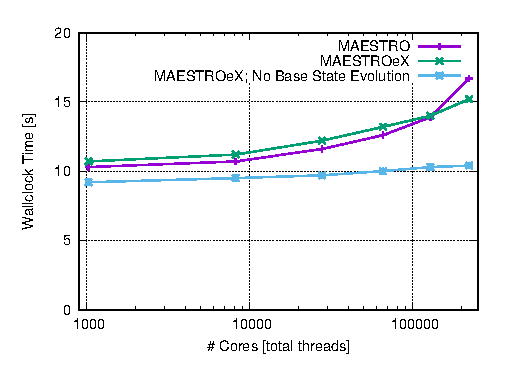
\includegraphics[width=2.75in]{./figs/MAESTRO_scaling1}
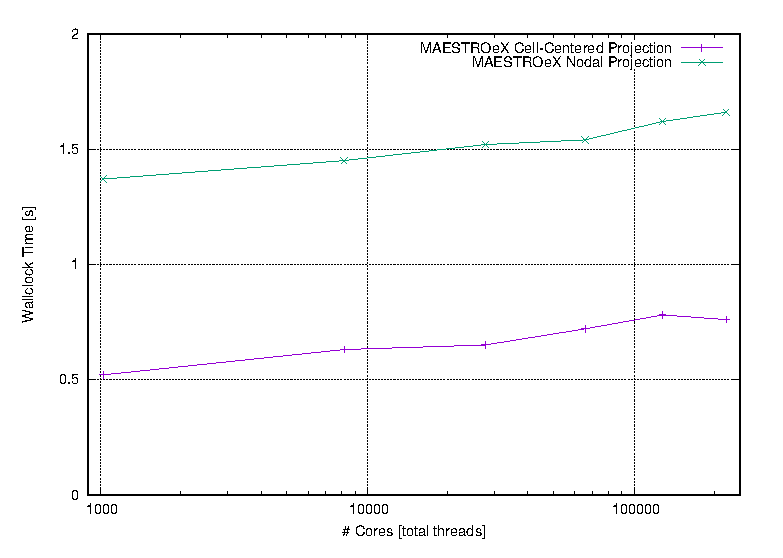
\includegraphics[width=2.75in]{./figs/MAESTRO_scaling2}
\caption{\label{fig:scaling} (Left) Weak scaling results for a spherical, full-star sub-Chandrasekhar mass white dwarf calculation using the original MAESTRO code, MAESTROeX, and MAESTROeX with base state evolution disabled.  Shown is the average wallclock time per time step.
(Right) Weak scaling results showing the average wallclock time per time step spent in the cell-centered and nodal linear solvers within a full time step of the aforementioned simulations.}
\end{center}
\end{figure}
%%%%%%%%%%%%%%%%%%%%%%%%%%%%%

In the left panel of Figure \ref{fig:scaling} we compare the wallclock time per time step as a function of total core count (in this case, the total number of OpenMP threads) for the original FBoxLib-based MAESTRO implementation to the AMReX MAESTROeX implementation.
These tests were performed using the original temporal integration strategy in \cite{MAESTRO_V}, noting that the new temporal integration with and without the irregular base state gives essentially the same results.
We also include a plot of MAESTROeX without base state evolution.
Comparing the original and new implementations, we see similar scaling results except for the largest simulation, where MAESTROeX performs better.
We see that the increase in wallclock time from the smallest to largest simulation is roughly 42\%.
We also note that without base state evolution, the code runs 14\% faster for small problems, and scale mush better
However, for the case without base state evolution, the overall runtime is faster and the increase in wallclock time from the smallest to largest simulation is roughly 13\%.
This is quite remarkable since there are 3 linear solver per time step (2 cell-centered Poisson solves used in the MAC projection, and a nodal Poisson solve used to compute the updated cell-centered velocities).
Contrary to our prior assumptions, the linear solves are not the primary scaling bottleneck in this code.
In the right panel of Figure \ref{fig:scaling}, we isolate the wallclock time required for these linear solves and see that (i) the linear solves only use 20-23\% of the total computational time, and (ii) the increase in the solver wallclock time from the smallest to largest simulation is only 28\%.
Further profiling reveals that the primary scaling bottleneck is the average operator.
The averaging operator requires binning the sum of Cartesian data onto one-dimensional arrays holding every possible mapping radius.
This amounts to at least 24,384 double precision values (for the $256^3$ simulation) up to 883,584 values (for the $1536^3$ simulation).
The averaging operator requires a global sum reduction over all processors, and the communication of this data is the primary scaling bottleneck.
For the simulation with base state evolution, this averaging operator is only called once per time step (as opposed to 14 times per time step when base state evolution is included).
The difference in total wallclock times with and without base state evolution is almost entirely due to the averaging.
Note that as expected, advection, reactions, and calls to the equation of state scale almost perfectly, since there is only a single parallel communication call to fill ghost cells.

\subsection{AMR Performance}
Show 3D reacting bubble rise performance.
Show 3-level spherical performance (stats won't be as good but explain why: refining a larger percentage of grid)
Images of grid configuration.

\subsection{White Dwarf Convection}
white dwarf convection runs with 3 algorithms (original, new temporal, new temporal + irregular base state)

Show 3-level wdconvect


\section{Conclusions and Future Work}

science: rotation, Urca, solar physics, MHD

algorithm: SDC \cite{dutt2000spectral}, high-order, multi-implicit \cite{bourlioux2003high}.
Consider SDC ideas used for terrestrial combustion \cite{pazner2016high,nonaka2018conservative}

implementation: GPUs.  Forward cite next CASTRO paper with GPU strategy.

\acknowledgements

The work at LBNL was supported by the U.S. Department of Energy's Scientific Discovery Through Advanced Computing (SciDAC) program under contract No. DE-AC02-05CH11231.
This research used resources of the National Energy Research Scientific Computing Center (NERSC), a U.S. Department of Energy Office of Science User Facility operated under Contract No. DE-AC02-05CH11231.


\appendix
\section{Projection Details}\label{Sec:Projection}
To enforce the divergence constraint in {\bf Step 3, 7}, and {\bf 11}, we use a projection method analgous to the methods originally developed for incompressible flow \citep{almgren1998conservative,bell1989second}.
The basic idea is to decompose the velocity field into a divergence-free component and a curl-free (gradient of a scalar field) component by solving a variable-coefficient Poisson equation for the scalar field.
The details for the MAC projection in {\bf Step 3} and {\bf Step 7} are given in Appendix B of Paper III.  The details of the nodal projection in {\bf Step 11} are given in Section 3.2 of Paper III.
We note that in the nodal projection, the gradient of the scalar field is used to update the perturbational pressure, $\pi$.

Based on our past experience in the MAESTRO project, we have found it useful to split the velocity dynamics into a perturbational and base state velocity,
\begin{equation}
\Ub = \Ubt(\xb,t) + w_0(r,t)\eb_r,
\end{equation}
solve for each term separately, and immediately combine them to find a full velocity that satisfies the constraint.  We take that approach here, primarily because it allows us to enforce a boundary condition on $w_0$ at the edge of the star (i.e., the cutoff density location where we hold density constant).  Namely, to enforce that $r^2 w_0$ remain constant is difficult to do when solving for the full velocity. 
This is demonstrated in Figure \ref{fig:wdconvect_splitU} (right) where the velocity magnitude is observed to incorrectly increase outside the cutoff density radius when we use the full velocity in the nodal projection. The resulting peak temperature also dips significantly as seen in Figure \ref{fig:wdconvect_splitU} (left).   

%%%%%%%%%%%%%%%%%%%%%%%%%%%%%
\begin{figure}[htb]
\begin{center}
\begin{tabular}{l r}
\multirow{4}{3.5in}[34.5mm]{ 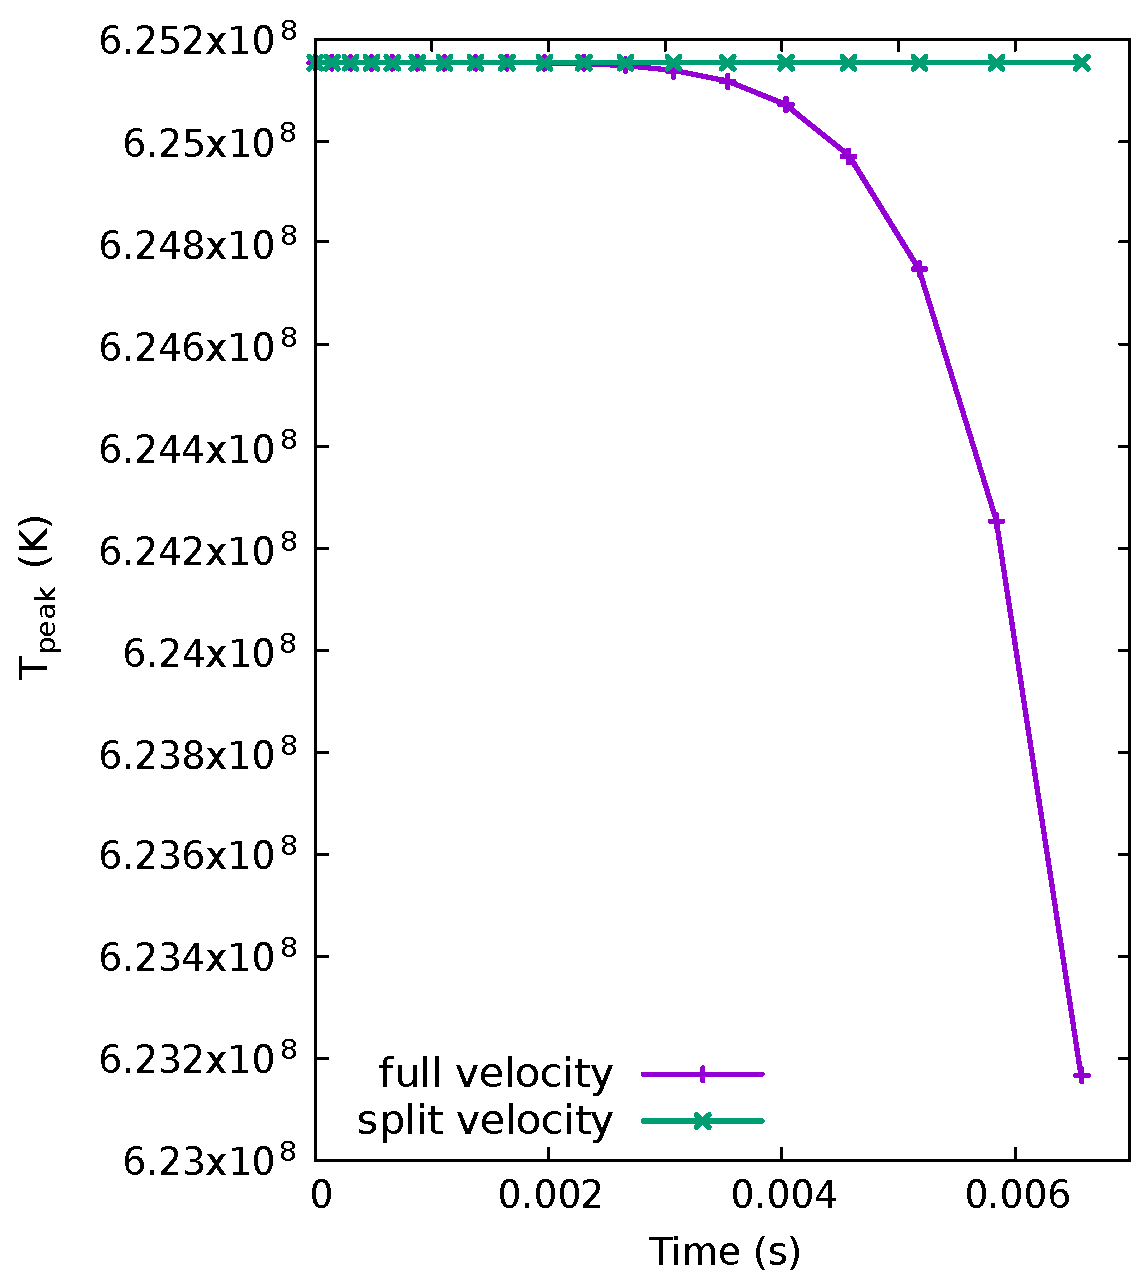
\includegraphics[width=3.0in]{./figs/wdconvect_256_splitU} } & \multicolumn{1}{c}{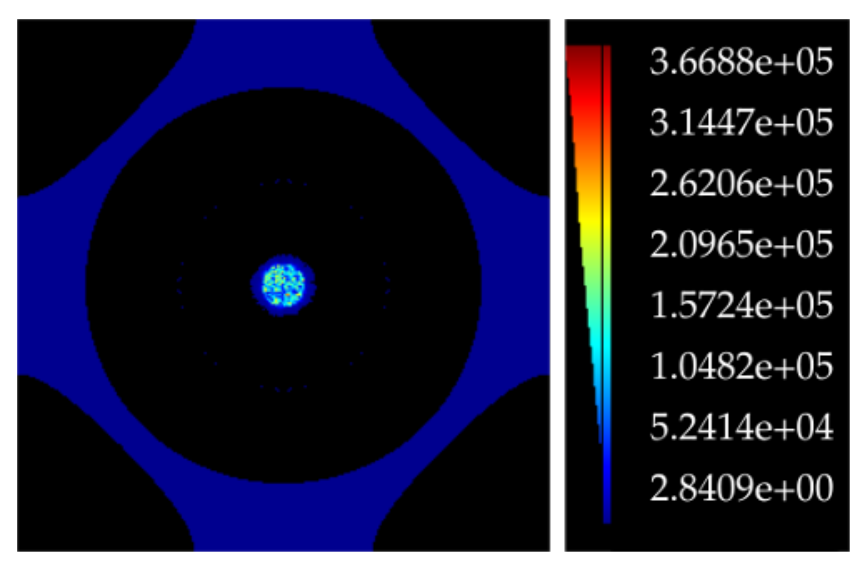
\includegraphics[width=2.35in]{./figs/magvel_full_XY}} \\
& \multicolumn{1}{c}{\begin{footnotesize} (a) $|\mathbf{U}|$, solved using $\mathbf{U}$ \end{footnotesize}} \\[1.em]
& \multicolumn{1}{c}{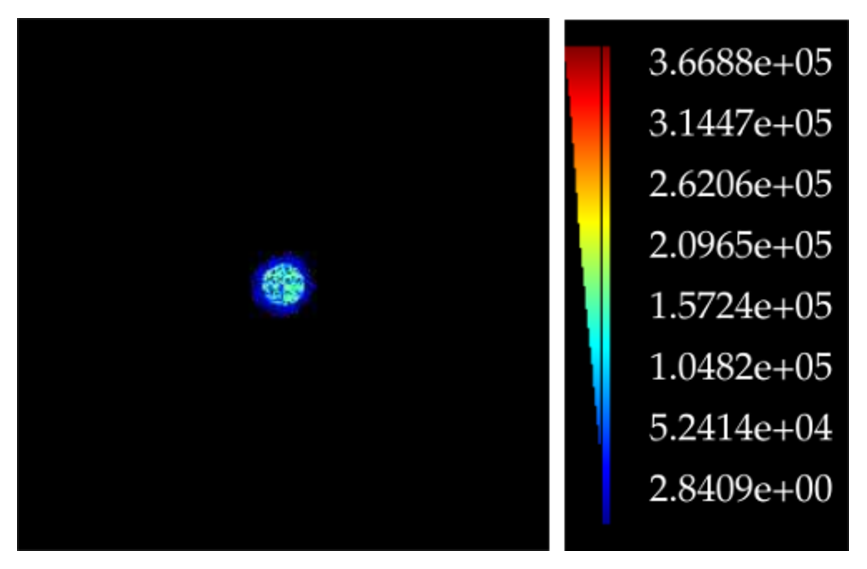
\includegraphics[width=2.35in]{./figs/magvel_split_XY}} \\ 
& \multicolumn{1}{c}{\begin{footnotesize} (b) $|\mathbf{U}|$, solved using $\tilde{\mathbf{U}}+w_0$ \end{footnotesize}} \\
\end{tabular}
\caption{\label{fig:wdconvect_splitU} (Left) Peak temperature, $T_{\text{peak}}$ in a white dwarf at resolution of $256^3$ 
         during initial transition. (Right) Velocity magnitude solved using full velocity $\mathbf{U}$ in the projection step 
         results in large values outside the density cutoff region that is not seen when we split the velocity dynamics.}
\end{center}
\end{figure}
%%%%%%%%%%%%%%%%%%%%%%%%%%%%%

So in practice, we solve the constraint over the lateral average,
\begin{equation}
\nabla\cdot\left(\beta_0\Ubt\right) = \beta_0(S-\overline{S})
\end{equation}
and separately solve for $w_0$ using 
\begin{equation}
\nabla\cdot(\beta_0w_0\eb_r) = \beta_0\left(\overline{S} - \frac{1}{\gammaonebar p_0}\frac{\partial p_0}{\partial t}\right).
\end{equation}
To solve for $\Ubt$ we use a projection method, which involves the solution of a variable-coefficient Poisson solver to extract the curl-free component of the unprojected velocity.
Note that MAESTRO contains alternate low Mach number formulations that conserve total energy in stratified systems, with minimal changes to the code (see Appendix A of \cite{subChandra_II} for details).
To find $w_0$ we integrate in 1D using the procedure in Appendix B of Paper V, keeping in mind that the base state spacing ($\Delta r$) should be computed using the appropriate cell-edge and cell-center locations when using irregularly-spaced base state.
Note that in this approach, we estimated the time-derivative of the pressure in part by examining how laterally averaged $\rho'=\rho-\rho_0$ changed over time (quantified by $\eta_\rho = \overline{\rho'\Ub\cdot\eb_r}$).  After evolving the species ({\bf Steps 4A/8A}), we compute this term in a similar fashion as reported in Paper V with the slight difference in using the full velocity instead of the split velocities. For example, after {\bf Step 8A}, we define a radial cell-centered $\etarho^{\nph}$, 

\begin{description}
\item For planar geometry, $\etarho = \overline{\rho'(\Ub\cdot\eb_r)}$,
\begin{equation}
 \etarho^{\nph} =  {\rm {\bf Average}} \sum_k \left[ \left(\uadvtwo \cdot \eb_r \right) (\rho X_k)^{\nph,\pred} \right]
\end{equation}
\item For spherical geometry, first construct 
$\etarho^{{\rm cart},\nph} = [\rho'(\Ub\cdot\eb_r)]^{\nph}$ on Cartesian cell centers using:
\begin{equation}
\etarho^{{\rm cart},\nph} = \left[\left(\frac{\rho^{(1)}+\rho^{(2)}}{2}\right)-\left(\frac{\rho_0^n+\rho_0^{n+1}}{2}\right)\right] \cdot \left( \uadvtwo \cdot \eb_r \right).
\end{equation}
Then,
\begin{equation}
\etarho^{\nph,\star} = {\rm {\bf Average}}\left(\etarho^{{\rm cart},\nph}\right).
\end{equation}
\end{description}





\bibliographystyle{aasjournal.bst}
\bibliography{references}

\end{document}
